\documentclass[10pt, portrait]{article}
\usepackage[scaled=0.92]{helvet}
\usepackage{calc}
\usepackage{multicol}
\usepackage{ifthen}
\usepackage[a4paper,margin=5mm,portrait]{geometry}
\usepackage{amsmath,amsthm,amsfonts,amssymb}
\usepackage{color,graphicx,overpic}
\usepackage{hyperref}
\usepackage{newtxtext} 
\usepackage{enumitem}
\usepackage{amssymb}
\usepackage[table]{xcolor}
\usepackage{vwcol}
\usepackage{tikz}
\usetikzlibrary{arrows.meta}
\usetikzlibrary{calc}
\usepackage{mathtools}
\usepackage{nicematrix}
\usepackage[T1]{fontenc} %%% <--- NOTE THIS
% for relations
\usepackage{cancel}
\usepackage{ mathrsfs }
\usepackage{listings}
\usepackage{background}
\setlist{nosep}

\backgroundsetup{
scale=1,
color=black,
opacity=0.3,
angle=0,
contents={%
  
\includegraphics[width=\paperwidth,height=\paperheight]{tantc.jpg}
  }%
}

\pdfinfo{
  /Title (CS1231S.pdf)
  /Creator (TeX)
  /Producer (pdfTeX 1.40.0)
  /Author (Seamus)
  /Subject (Example)
  /Keywords (pdflatex, latex,pdftex,tex)}

\lstset{language=Java,keywordstyle={\bfseries \color{black}}}

% Turn off header and footer
\pagestyle{empty}

\newenvironment{tightcenter}{%
  \setlength\topsep{0pt}
  \setlength\parskip{0pt}
  \begin{center}
}{%
  \end{center}
}

% redefine section commands to use less space
\makeatletter
\renewcommand{\section}{\@startsection{section}{1}{0mm}%
                                {-1ex plus -.5ex minus -.2ex}%
                                {0.5ex plus .2ex}%x
                                {\normalfont\large\bfseries}}
\renewcommand{\section}{\@startsection{section}{2}{0mm}%
                                {-1explus -.5ex minus -.2ex}%
                                {0.5ex plus .2ex}%
                                {\normalfont\normalsize\bfseries}}
\renewcommand{\subsection}{\@startsection{subsection}{3}{0mm}%
                                {-1ex plus -.5ex minus -.2ex}%
                                {1ex plus .2ex}%
                                {\normalfont\small\bfseries}}%
\renewcommand{\familydefault}{\sfdefault}
\renewcommand\rmdefault{\sfdefault}
% makes nested numbering (e.g. 1.1.1, 1.1.2, etc)
\renewcommand{\labelenumii}{\theenumii}
\renewcommand{\theenumii}{\theenumi.\arabic{enumii}.}
\renewcommand\labelitemii{•}
%  for logical not operator
\renewcommand{\lnot}{\mathord{\sim}}
\renewcommand{\bf}[1]{\textbf{#1}}
\newcommand{\abs}[1]{\vert #1 \vert}
\newcommand{\Mod}[1]{\ \mathrm{mod}\ #1}

\makeatother
\definecolor{myblue}{cmyk}{1,.72,0,.38}
\everymath\expandafter{\the\everymath \color{myblue}}
% Define BibTeX command
\def\BibTeX{{\rm B\kern-.05em{\sc i\kern-.025em b}\kern-.08em
    T\kern-.1667em\lower.7ex\hbox{E}\kern-.125emX}}
\let\iff\leftrightarrow
\let\Iff\Leftrightarrow
\let\then\rightarrow
\let\Then\Rightarrow

% Don't print section numbers
\setcounter{secnumdepth}{0}

\setlength{\parindent}{0pt}
\setlength{\parskip}{0pt plus 0.5ex}
%% this changes all items (enumerate and itemize)
\setlength{\leftmargini}{0.5cm}
\setlength{\leftmarginii}{0.5cm}
\setlist[itemize,1]{leftmargin=2mm,labelindent=1mm,labelsep=1mm}
\setlist[itemize,2]{leftmargin=4mm,labelindent=1mm,labelsep=1mm}

%My Environments
\newtheorem{example}[section]{Example}
% -----------------------------------------------------------------------

\begin{document}
\raggedright
\footnotesize
\begin{multicols*}{2}


% multicol parameters
% These lengths are set only within the two main columns
\setlength{\columnseprule}{0.25pt}
\setlength{\premulticols}{1pt}
\setlength{\postmulticols}{1pt}
\setlength{\multicolsep}{1pt}
\setlength{\columnsep}{2pt}

\begin{center}
    \fbox{%
        \parbox{0.8\linewidth}{\centering \textcolor{black}{
            {\Large\textbf{CS1231S}}
            \\ \normalsize{AY24/25 Sem 1}}
            \\ {\footnotesize \textcolor{myblue}{by ngmh}} 
        }%
    }
\end{center}

\section{1. Speaking Mathematically}
\subsection{Important Sets}
\begin{itemize}
    \item $\mathbb{N}$: the set of all natural numbers (include $0$, i.e. $\mathbb{Z}_{\ge 0}$)
    \item $\mathbb{Z}$: the set of all integers
    \item $\mathbb{Q}$: the set of all rational numbers
    \item $\mathbb{R}$: the set of all real numbers
    \item $\mathbb{C}$: the set of all complex numbers
\end{itemize}

\subsection{Statements}
\begin{itemize}
    \item Universal Statement $\forall$: A certain property is true for \textbf{all} elements in a set
    \item Conditional statement $\rightarrow$: If one thing is true then some other thing has to be true
    \item Existential Statement $\exists$: There is \textbf{at least one} thing for which a certain property is true
    \item Universal Conditional Statement
    \item Universal Existential Statement
    \item Existential Universal Statement (not the same!)
\end{itemize}

\subsection{Terms used in Proofs}
\begin{itemize}
    \item Definition: Precise and unambiguous description of mathematical term.
    \item Axiom / Postulate: A statement that is assumed to be true without proof.
    \item Theorem: A mathematical statement that is proved using rigorous mathematical reasoning.
    \item Lemma: A small theorem; a minor result which helps to prove a theorem.
    \item Corollary: A result that is a simple deduction from a theorem.
    \item Conjecture: A statement believed to be true, but for which there is no proof (yet).
\end{itemize}

\subsection{Properties of Integers on Addition and Multiplication}
\begin{itemize}
    \item Closure: $x+y \in \mathbb{Z}$
    \item Commutativity: $x+y = y+x$
    \item Associativity: $x+y+z = (x+y)+z = x+(y+z)$
    \item Distributivity: $x(y+z) = xy + xz$
    \item Trichotomy: $x = y$ or $x < y$ or $x > y$
\end{itemize}

\subsection{Number Definitions}
\begin{itemize}
    \item Even and Odd Integers (Lecture 1 Slide 27): An integer is even iff $\exists k s.t. n = 2k$. An integer is odd iff $\exists k s.t. n = 2k+1$. Every integer is even or odd, but not both (Assumption 1).
    \item Without Loss Of Generality (WLOG): Used before an assumption in a proof which narrows the premise to some special case, and implies that the proof for that case can be easily applied to all other cases.
    \item Counter-Example: Shows that a statement is not always true.
    \item Divisibility (Lecture 1 Slide 32): If n and d are integers with $d \neq 0$, $d \mid n$ iff $\exists k \in \mathbb{Z}$ s.t. $n = dk$
    \item Theorem 4.7.1: $\sqrt{2}$ is irrational
    \item Rational and Irrational Numbers: r is rational iff $\exists a, b \in \mathbb{Z}$ s.t. $r = \frac{a}{b}, b \neq 0$
    \item Fraction in lowest term (Lecture 1 Slide 37): A fraction $\frac{a}{b}$ is said to be in lowest terms if the largest integer that divides both a and b is 1. Every rational can be reduced to a fraction in its lowest term. (Assumption 2)
    \item Proposition 4.6.4: For all integers $n$, if $n^2$ is even then $n$ is even. (Proof by contraposition)
    \item Colorful (CS1231S): An integer $n$ is colorful if $\exists k$ s.t. $n = 3k$
\end{itemize}

\section{2. The Logic of Compound Statements}
\subsection{Definitions}
\begin{itemize}
    \item Defn 2.1.1 (Statement): A statement (or proposition) is a sentence that is true or false, but not both.
    \item Defn 2.1.2 (Negation): The negation of p is "not p" and is denoted $\lnot p$.
    \item Defn 2.1.3 (Conjunction): The conjunction of p and q is "p and q", denoted $p \land q$.
    \item Defn 2.1.4 (Disjunction): The disjunction of p and q is "p or q", denoted $p \lor q$.
    \item Defn 2.1.5 (Statement Form / Propositional Form): A statement form (or propositional form) is an expression made up of statement variables and logical connectives.
    \item Defn 2.1.6 (Logical Equivalence): Two statement forms are logically equivalent iff they have identical truth values for each possible substitution of statements for their statement variables. The logical equivalence of P and Q is denoted by $P \equiv Q$.
    \item Defn 2.1.7 (Tautology): A tautology is a statement form that is always true regardless of the truth values of its statement variables.
    \item Defn 2.1.8 (Contradiction): A contradiction is a statement form that is always false regardless of the truth values of its statement variables.
    \item Defn 2.2.1 (Conditional): The conditional of q by p is "if p then q", denoted $p \rightarrow q$. p is the hypothesis (antecedent), and q is the conclusion (consequent).
    \item Defn 2.2.2 (Contrapositive): The contrapositive of a conditional statement $p \rightarrow q$ is $\lnot q \rightarrow \lnot p$
    \item Defn 2.2.3 (Converse): The converse of a conditional statement $p \rightarrow q$ is $q \rightarrow p$ 
    \item Defn 2.2.4 (Inverse): The inverse of a conditional statement $p \rightarrow q$ is $\lnot p \rightarrow \lnot q$ 
    \item Defn 2.2.5 (Only if): "p only if q" means $\lnot q \rightarrow \lnot p$ or "if p then q" $p \rightarrow q$
    \item Defn 2.2.6 (Biconditional): The biconditional of p and q is "p if and only if q" and is denoted "$p \leftrightarrow q$"
    \item Defn 2.2.7 (Necessary and Sufficient Conditions): "r is a sufficient condition for s" means $r \rightarrow s$, "r is a necessary condition for s" means $s \rightarrow r$
    \item Defn 2.3.1 (Argument): An argument is a sequence of statements. All statements except for the final one are called premises, while the final statement is called the conclusion. The symbol $\therefore$ is normally placed before the conclusion. An argument form is valid if the conclusion is true when all the premises are true.
    \item Defn 2.3.2 (Sound and Unsound Arguments): an argument is sound iff it is valid and all its premises are true. An argument that is not sound is unsound.
\end{itemize}

\subsection{Theorem 2.1.1 Logical Equivalences}
\begin{multicols*}{2}
Implication Law
$$p \rightarrow q \equiv \lnot p \lor q$$
Commutative Laws
  $$ p \land q \equiv q \land p $$
  $$ p \lor  q \equiv q \lor  p $$
Associative Laws
  $$ p \land q \land r \equiv (p \land q) \land r \equiv p \land (q \land r) $$
  $$ p \lor q \lor r \equiv (p \lor  q) \lor  r \equiv p \lor  (q \lor  r) $$
Distributive Laws
  $$ p \land (q \lor  r) \equiv (p \land q) \lor  (p \land r) $$
  $$ p \lor  (q \land r) \equiv (p \lor  q) \land (p \lor  r) $$
Identity Laws
  $$ p \land \textbf{true} \equiv p $$
  $$ p \lor  \textbf{false} \equiv p $$
Negation Laws
  $$ p \lor  \lnot p \equiv \textbf{true} $$
  $$ p \land \lnot p \equiv \textbf{false} $$
Double Negative Law
  $$ \lnot ( \lnot p ) \equiv p $$
Idempotent Laws
  $$ p \land p \equiv p $$
  $$ p \lor  p \equiv p $$
Universal Bound Laws
  $$ p \lor  \textbf{true} \equiv \textbf{true} $$
  $$ p \land \textbf{false} \equiv \textbf{false} $$
De Morgan's Laws
  $$ \lnot ( p \land q ) \equiv \lnot p \lor  \lnot q $$
  $$ \lnot ( p \lor  q ) \equiv \lnot p \land \lnot q $$
Absorption Laws
  $$ p \lor  (p \land q) \equiv p $$
  $$ p \land (p \lor  q) \equiv p $$
Negations of $\textbf{true}$ and $\textbf{false}$
  $$ \lnot \textbf{true} \equiv \textbf{false} $$
  $$ \lnot \textbf{false} \equiv \textbf{true} $$
\end{multicols*}

\subsection{Argument Forms and Fallacies}
\begin{multicols*}{2}
\begin{itemize}
    \item Modus Ponens:
    \begin{itemize}
        \item If $p$ then $q$
        \item $p$
        \item $\therefore q$
    \end{itemize}
    \item Modus Tollens:
    \begin{itemize}
        \item If $p$ then $q$
        \item $\lnot q$
        \item $\therefore \lnot p$
    \end{itemize}
    \item Generalization:
    \begin{itemize}
        \item $p$
        \item $p \lor q$
    \end{itemize}
    \item Specialization:
    \begin{itemize}
        \item $p \land q$
        \item $\therefore p$
    \end{itemize}
    \item Conjunction:
    \begin{itemize}
        \item $p$
        \item $q$
        \item $\therefore p \land q$
    \end{itemize}
    \item Elimination:
    \begin{itemize}
        \item $p \lor q$
        \item $\lnot q$
        \item $\therefore p$
    \end{itemize}
    \item Transitivity:
    \begin{itemize}
        \item $p \rightarrow q$
        \item $q \rightarrow r$
        \item $\therefore p \rightarrow r$
    \end{itemize}
    \item Division into Cases
    \begin{itemize}
        \item $p \lor q$
        \item $p \rightarrow r$
        \item $q \rightarrow r$
        \item $\therefore r$
    \end{itemize}
    \item Contradiction Rule
    \begin{itemize}
        \item $\lnot p \rightarrow false$
        \item $\therefore p$
    \end{itemize}
    \item Converse Error
    \begin{itemize}
        \item $p \rightarrow q$
        \item $q$
        \item $p$
    \end{itemize}
    \item Inverse Error
    \begin{itemize}
        \item $p \rightarrow q$
        \item $\lnot p$
        \item $\lnot q$
    \end{itemize}
\end{itemize}
\end{multicols*}

\subsection{Compund Statements Notes}
\begin{itemize}
     \item Order of Operations: $\lnot, \land / \lor, \rightarrow / \leftrightarrow$ \ (use parentheses if ambiguous)
    \item Show logical unequivalence by (i) finding a different row in truth table, (ii) finding a counter example.
    \item A conditional statement is vacuously true when the hypothesis is false.
    \item A conditional is logically equivalent with its contrapositive, which is the negation of its converse / inverse.
    \item If r is a sufficient condition for s, then r is sufficient to guarantee the occurrence of r.
    \item If r is a necessary condition for s, s cannot occur without r.
    \item To test an argument form for validity, construct the truth table. A critical row is a row in the truth table in which all premises are true. If there is a critical row in which the conclusion is false, the argument form is invalid. If there are no critical rows, the argument is vacuously valid.
\end{itemize}

\section{3. The Logic of Quantified Statements}
\subsection{Definitions}
\begin{itemize}
    \item Defn 3.1.1 (Predicate): A predicate is a sentence that contains a finite number of variables and becomes a statement when specific values are substituted for the variables. The domain of a predicate variable is the set of all values that may be substituted in place of the variable.
    \item Defn 3.1.2 (Truth Set): If $P(x)$ is a predicate and $x$ has domain $D$, the truth set has all elements of $D$ that make $P(x)$ true when substituted for x, denoted by $\{x \in D \mid P(x)\}$
    \item Defn 3.1.3 (Universal Statement): Let $Q(x)$ be a predicate and $D$ the domain of $x$. A universal statement has the form $\forall x \in D, Q(x)$. A value for $x$ for which $Q(x)$ is false is a counterexample.
    \item Defn 3.1.4 (Existential Statement): Let $Q(x)$ be a predicate and $D$ the domain of $x$. An existential statement has the form $\exists x \in D$ s.t. $Q(x)$. The symbol $\exists !$ is used to denote uniqueness.
    \item Theorem 3.2.1 Negation of a Universal Statment: The negation of the statement $\forall x \in D, P(x)$ is equivalent to $\exists x \in D$  s.t. $\lnot P(x)$
    \item Theorem 3.2.2 Negation of an Existential Statement: The negation of the statment $\exists x \in D$ s.t. $P(x)$ is equivalent to $\forall x \in D, \lnot P(x)$
    \item Defn 3.2.1 (Contrapositive, Converse, Inverse): These terms can also be applied on universal conditional statements.
    \item Defn 3.2.2 (Necessary and Sufficient conditions, Only if): These terms can also be applied on universal conditional statements.
    \item Defn 3.4.1 (Valid Argument Form): An argument form is valid if no matter what predicates are substituted in its premises, if the premise statements are all true, then the conclusion is also true. An argument is valid iff its form is valid.
\end{itemize}

\subsection{Arguments with Quantified Statements}
\begin{multicols*}{2}
\begin{itemize}
    \item Universal Modus Ponens:
    \begin{itemize}
        \item $\forall x (P(x) \rightarrow Q(x))$
        \item $P(a)$ for a particular $a$
        \item $\therefore Q(a)$
    \end{itemize}
    \item Universal Modus Tollens
    \begin{itemize}
        \item $\forall x, (P(x) \rightarrow Q(x)$
        \item $\lnot Q(a)$ for a particular $a$
        \item $\therefore \lnot P(a)$
    \end{itemize}
    \item Universal Transitivity
    \begin{itemize}
        \item $\forall x (P(x) \rightarrow Q(x)$
        \item $\forall x (Q(x) \rightarrow R(x)$
        \item $\therefore \forall x (P(x) \rightarrow R(x)$
    \end{itemize}
    \item Universal Instantiation
    \begin{itemize}
        \item $\forall x \in D P(x)$
        \item $\therefore P(a)$ if $a \in D$
    \end{itemize}
    \item Universal Generalisation
    \begin{itemize}
        \item $P(a)$ for every $a \in D$
        \item $\therefore \forall x \in D P(x)$
    \end{itemize}
    \item Existential Instantiation
    \begin{itemize}
        \item $\exists x \in D P(x)$
        \item $\therefore P(a)$ for some  $a \in D$
    \end{itemize}
    \item Existential Generalisation
    \begin{itemize}
        \item $P(a)$ for some $a \in D$
        \item $\exists x \in D P(x)$
    \end{itemize}
    \item Converse Error
    \begin{itemize}
        \item $\forall x (P(x) \rightarrow Q(x))$
        \item $Q(a)$ for a particular $a$
        \item $\therefore P(a)$
    \end{itemize}
    \item Inverse Error
    \begin{itemize}
        \item $\forall x (P(x) \rightarrow Q(x))$
        \item $\lnot P(a)$ for a particular $a$
        \item $\therefore \lnot Q(a)$
    \end{itemize}
\end{itemize}
\end{multicols*}

\subsection{Quantified Statements Notes}
\begin{itemize}
    \item To show a universal statement is true, we use exhaustion. To show it is false, we use a counterexample.
    \item To show an existential statement is true, we use an example. To show it is false, we use exhaustion.
    \item $\forall x \in D, Q(x) \equiv Q(x_1) \land Q(x_2) \land ... \land Q(x_n)$, and $\exists x \in D, Q(x) \equiv Q(x_1) \lor Q(x_2) \lor ... \lor Q(x_n)$
    \item Universal statements can be vacuously true if the predicate of a conditional is false for every element in the domain, which also happens if the domain is empty.
    \item In a statement with multiple quantifiers, the order of quantifiers with the \textbf{SAME} type can be interchanged.
\end{itemize}

\section{4. Methods of Proof}
\subsection{Definitions}
\begin{itemize}
    \item Prime: An integer $n$ is prime iff $n > 1$ and $\forall r, s$, if $n = rs$ then $r = n$ or $s = n$.
    \item Composite: An integer $n$ is composite iff $n > 1$ and $\exists r, s$ s.t. $n = rs$, $1 < r < n$, $1 < s < n$.
    \item Theorem 4.2.1: Every integer is a rational number. (Prove with $\frac{a}{1}$)
    \item Theorem 4.2.2: The sum of any two rational numbers is rational. (Proof by algebra)
    \item Corollary 4.2.3: The double of a rational number is rational.
    \item Theorem 4.3.1: $\forall a, b$, if $a \mid b$ then $a \leq b$ (Proof by algebra)
    \item Theorem 4.3.2: The only divisors of 1 are 1 and -1 (Proof by cases)
    \item Theorem 4.3.3: $\forall a, b, c$ if $a \mid b$ and $b \mid c$ then $a \mid c$
    \item Theorem 4.6.1: There is no greatest integer (Proof by contradiction)
\end{itemize}

\subsection{Proofs}

\subsection{Methods of Proof}
\begin{itemize}
    \item Direct Proof: Show a series of steps leading from start to end. Deduction is a type of direct proof.
    \item Divison into Cases: Split the statement into cases and show it is true in all of them.
    \item Constructive Proof of Existential statements: Provide an example where the statement is true.
    \item Disproving Universal Statements by Counterexample: Give a counterexample where the negation is true, or where the antecedent is true and the consequent is false.
    \item Proving Universal Statements by Exhaustion: Show the statement is true for every element in the domain.
    \item Proving Universal Statements by Generalizing from the Generic Particular: Suppose x is a particular but arbitrarily chosen element of the set, show x satisfies the property.
    \item Proof by Contradiction:
    \begin{itemize}
        \item Suppose the statement to be proved, $S$, is false. That is, the negation of the statement, $\lnot S$, is true.
        \item Show that this supposition leads logically to a contradiction.
        \item Conclude that the statement $S$ is true.
    \end{itemize}
    \item Proof by Contraposition: Prove the contraposition of the statement instead.
\end{itemize}

\section{5. Set Theory}
\subsection{Definitions}
\begin{itemize}
    \item Set: An \textbf{unordered} collection of objects (members / elements)
    \item Set-Roster Notation: Write all elements of the set between braces.
    \item Membership of a set: $x \in S$ means $x$ is an element of $S$. Similarly, $x \notin S$ means $x$ is not an element of $S$.
    \item Cardinality of a set: $\mid S \mid$ is the size of the set $S$, or the number of elements in $S$.
    \item Set-Builder Notation: Let $U$ be a set and $P(x)$ be a predicate over $U$. Then the set of $x \in U$ s.t. $P(x)$ is true is $\{x \in U : P(x)\}$.
    \item Replacement Notation: Let $A$ be a set and $t(x)$ be a term in a variable $x$. Then the set of all objects of the form $t(x)$ where $x \in A$ is $\{t(x) : x \in A\}$.
    \item Subset and Superset: Let A and B be sets. A is a subset of B, $A \subseteq B$, iff every element in A is also an element of B. We can also write $B \supseteq A$ or B is a superset of A.
    \item Proper Subset: A is a proper subset of B, $A \subsetneq B$ iff $A \subseteq B$ and $A \neq B$.
    \item Empty Set: $\emptyset$
    \item Theorem 6.2.4: An empty set is a subset of every set, $\forall A, \emptyset \subseteq A$
    \item Singleton: Set with exactly one element.\
    \item Ordered Pair: An ordered pair has the form $(x, y)$. Two Ordered pairs $(a, b)$ and $(c, d)$ are equal iff $a = c$ and $b = d$. This can also be extended to ordered n-tuples.
    \item Cartesian Product: The Cartesian product of sets A and B, $A \times B$, is the set of all ordered pairs $(a, b)$ where $a \in A$ and $b \in B$. This can also be extended to more than 2 sets.
    \item Set Equality: $A = B$ iff every element of $A$ is $B$ and every element of $B$ is in $A$, or $A \subseteq B$ and $B \subseteq A$.
    \item Union: The union of $A$ and $B$, $A \cup B$ is the set of all elements that are in at least one of $A$ or $B$.
    \item Intersection: The intersection of $A$ and $B$, $A \cap B$ is the set of all elements that are in both $A$ and $B$.
    \item Difference / Relative Complement: The difference of $B - A$, $B \backslash A$ is the set of elements that are in $B$ and not $A$.
    \item Complement: The complement of $A$, $\bar{A}$ is the set of elemnts in $U$ that are not in $A$.
    \item Interval Notation: $(a, b) = \{x \in \mathbb{R} : a \textless x \textless b\}$, $[a, b] = \{x \in \mathbb{R} : a \leq x \leq b\}$. $[]$ means closed intervals, while $()$ means open intervals.
    \item Disjoint: Two sets are disjoint iff they have no elements in common, $A \cap B = \emptyset$.
    \item Mutually / Pairwise Disjoint / Nonoverlapping: Multiple sets are mutually disjoint iff $\forall A_i, A_j$, $A_i$ and $A_j$ are disjoint.
    \item Partition: Collection of mutually disjoint sets.
    \item Theorem 4.4.1 Quotient-Remainder Theorem: Given $n, d$, $\exists ! q, r$ s.t. $n = dq+r$, $0 \leq r \textless d$
    \item Power Set: $\mathcal{P}(A)$ is the set of all subsets of $A$. By power set axiom, any element of $\mathcal{P}(A)$ is a set.
    \item Theorem 6.3.1 Cardinality of Power Set of a Finite Set: If $\mid A \mid = n$, $\mid \mathcal{P}(A) \mid = 2^n$.
\end{itemize}

\subsection{Set Properties}
\begin{itemize}
    \item Inclusion of Intersection: $A \cap B \subseteq A$
    \item Inclusion in Union: $A \subseteq A \cup B$
    \item Transitive Property of Subsets: $A \subseteq B \land B \subseteq C \rightarrow A \subseteq C$.
    \item Procedural Definitions: Define using $\land, \lor$ instead
    \begin{itemize}
        \item $a \in X \cup Y \leftrightarrow a \in X \lor a \in Y$
        \item $a \in X \cap Y \leftrightarrow a \in X \land a \in Y$
        \item $a \in X - Y \leftrightarrow a \in X \land a \notin Y$
        \item $a \in \bar{X} \leftrightarrow a \notin X$
        \item $(a, b) \in X \times Y \leftrightarrow a \in X \land b \in Y$
    \end{itemize}
\end{itemize}

\subsection{Theorem 6.2.2 Set Identities}
\begin{multicols*}{2}
Commutative Laws
$$A \cup B = B \cup A$$
$$A \cap B = B \cap A$$
Associative Laws
$$(A \cup B) \cup C = A \cup (B \cup C)$$
$$(A \cap B) \cap C = A \cap (B \cap C)$$
Distributive Laws:
$$A \cup (B \cap C) = (A \cup B) \cap (A \cup C)$$
$$A \cap (B \cup C) = (A \cap B) \cup (A \cap C)$$
Identity Laws
$$A \cup \emptyset = A$$
$$A \cap U = A$$
Complement Laws
$$A \cup \bar{A} = U$$
$$A \cap \bar{A} = \emptyset$$
Double Complement Law
$$\bar{\bar{A}} = A$$
Idempotent Laws
$$A \cup A = A$$
$$A \cap A = A$$
Universal Bound Laws
$$A \cup U = U$$
$$A \cap \emptyset = \emptyset$$
De Morgan's Laws
$$\overline{A \cup B} = \bar{A} \cap \bar{B}$$
$$\overline{A \cap B} = \bar{A} \cup \bar{B}$$
Absorption Laws
$$A \cup (A \cap B) = A$$
$$A \cap (A \cup B) = A$$
Complements of $U$ and $\emptyset$
$$\bar{U} = \emptyset$$
$$\bar{\emptyset} = U$$
Set Difference Law
$$A \backslash B = A \cap \bar{B}$$
\end{multicols*}

\section{6. Relations}
\subsection{Definitions}
\begin{itemize}
    \item Relation: A binary relation from $A$ to $B$ is a subset of $A \times B$. Given an ordered pair $(x, y)$ in $A \times B$, $x$ is related to $y$ by $R$, $x R y$, iff $(x, y) \in R$
    \item Domain, Co-Domain, Range: Let $R$ be a relation from $A$ to $B$. Domain is the set $\{a \in A : a R b$ for some $b \in B\}$. Co-Domain is B. Range is the set $\{b \in B : a R b$ for some $a \in A\}$
    \item Inverse Relation: The inverse relation $R^{-1}$ is $\{(y, x) \in B \times A : (x, y) \in R\}$
    \item Relation on a Set: A relation on a set $A$ is a subset of $A \times A$.
    \item Composite Relations: Let $R \subseteq A \times B$ and $S \subseteq B \times C$ be relations. The composition of $R$ with $S$, denoted $S \circ R$ is the relation from $A$ to $C$ s.t. $\forall x \in A, \forall Z \in C, x S \circ R z \leftrightarrow (\exists y \in B, x R y \land y S z)$.
    \item Proposition: Composition is Associative
    \item Proposition: Inverse of Composition: $(S \circ R)^{-1} = R^{-1} \circ S^{-1}$.
    \item n-ary Relation: Subset of $A^n$
    \item Reflexivity: $R$ is reflexive iff $\forall x \in A, x R x$.
    \item Symmetry: $R$ is symmetric iff $\forall x, y \in A, x R y \rightarrow y R x$
    \item Antisymmetry: $R$ is antisymmetric iff $\forall x, y \in A, x R y \land y R x \rightarrow x = y$.
    \item Assymetry: $R$ is asymmetric iff $\forall x, y \in A, x R y \rightarrow y \cancel{R} x$
    \item Transitivity: $R$ is transitive iff $\forall x, y, z \in A, x R y \land y R z \rightarrow x R z$.
    \item Transitive Closure: The transitive closure of $R$ on $A$ is $R^t$ on $A$ s.t. (i) $R^t$ is transitive, (ii) $R \subseteq R^t$, (iii) If $S$ is another transitive relation containing $R$, $R^t \supseteq S$. Reflexive and Symmetric closure are similarly defined.
    \item Partition: $\mathscr{C}$ is a partition of $A$ if (i) $\mathscr{C}$ is a set where all elements are non-empty subsets of $A$, (ii) Every element of $A$ is in exactly one element of $\mathscr{C}$. Elements of a partition are components. Alternatively, $\forall x \in A, \exists ! S \in \mathscr{C} (x \in S)$.
    \item Relation Induced by Partition: The relation $R$ induced by a partition on $A$ is $\forall x, y, \in A, x R y \leftrightarrow \exists$ a component $S$ of $\mathscr{C}$ s.t. $x, y, \in S$.
    \item Theorem 8.3.1 Relation Induced by a Partition: $R$ is reflexive, symmetric, and transitive.
    \item Equivalence Relation: $R$ is an equivalence relation iff $R$ is reflexive, symmetric and transitive. The symbol $\lnot$ is commonly used.
    \item Equivalence Class: Suppose $A$ is a set and $\lnot$ is an equivalence relation on $A$. For each $a \in A$, the equivalence class of $a$, $[a]$, is the set of elements $x \in A$ s.t. $a \lnot x$. $[a]_{\lnot} = \{x \in A : a \lnot x\}$
    \item Theorem 8.3.4: The partition Induced by an Equivalence Relation: If $R$ is an equivalence relation on $A$, then the distinct equivalence classes of $R$ form a partition of $A$.
    \item Congruence: $a$ is congruent to $b$ modulo $n$ iff $a-b = nk$ for some $k \in \mathbb{Z}$.
    \item Congruence mod $n$ is an equivalence relation on $\mathbb{Z}$ for every $n \in \mathbb{Z}^+$
    \item Set of equivalence classes: $A / \lnot$ is the set of all equivalence classes with respect to $\lnot$, $A / \lnot = \{[x]_{\lnot} : x \in A\}$.
    \item Partial Order Relation: $R$ is a partial order iff $R$ is reflexive, antisymmetric and transitive.
    \item Partially Ordered Set: $A$ is a poset with respect to a partial order relation $R$ on $A$, $(A, R)$.
    \item Curly Less Than Equals: $\preccurlyeq$ is used for partial orders to prevent confusion with $\leq$.
    \item Hasse Diagrams: Simplification of the directed graph of a partial order relation. Place vertices s.t. all arrows point upwards, then remove all self-loops, remove arrows implied by transitivity, and remove direction indicators.
    \item Comparable: $a$ and $b$ are comparable iff $a \preccurlyeq b$ or $b \preccurlyeq a$. If not, they are noncomparable.
    \item Compatible: $a$ and $b$ are compatible iff $\exists c \in A, a \preccurlyeq c, b \preccurlyeq c$. (There are other possible definitions, be careful.)
    \item Maximal Element: $c$ is maximal iff $\forall x \in A, c \preccurlyeq x \rightarrow c = x$.
    \item Minimal Element: $c$ is minimal iff $\forall x \in A, x \preccurlyeq c \rightarrow c = x$.
    \item Largest Element: $c$ is the largest iff $\forall x \in A, x \preccurlyeq c$.
    \item Smallest Element: $c$ is the smallest iff $\forall x \in A, c \preccurlyeq x$.
    \item Total Order Relations: $R$ is a total order relation if $R$ is a partial order and $\forall x, y \in A, x R y \lor y R x$.
    \item Linearization: A total order s.t. $x \preccurlyeq y \rightarrow x \preccurlyeq^* y$.
    \item Well-Ordered Set: $A$ is well-ordered iff every non-empty subset of $A$ contains a smallest (not minimal) element.
\end{itemize}

\subsection{Lemma Rel.1 Equivalence Classes}
The following are equivalent:
\begin{itemize}
    \item (i) $x \lnot y$
    \item (ii) $[x] = [y]$
    \item (iii) $[x] \cap [y] \neq \emptyset$
\end{itemize}
Proof
\begin{itemize}
    \item (i) $\rightarrow (ii)$
    \begin{itemize}
        \item Suppose $x \lnot y$
        \item $y \lnot x$ by symmetry
        \item For every $z \in [x]$
        \item $x \lnot z$ by definition of $[x]$
        \item $y \lnot z$ by transitivity
        \item $z \in [y]$ by definition of $[y]$
        \item $\therefore [x] \subseteq [y]$
        \item Similarly for $[y] \subseteq [x]$
        \item $\therefore [x] = [y]$
    \end{itemize}
    \item (ii) $\rightarrow$ (iii)
    \begin{itemize}
        \item Suppose $[x] = [y]$
        \item $[x] \cap [y] = [x]$ by Idempotent Law
        \item However, $x \lnot x$ by reflexivity
        \item This shows $x \in [x] = [x] \cap [y]$
        \item $\therefore [x] \cap [y] \neq \emptyset$
    \end{itemize}
    \item (iii) $\rightarrow$ (i)
    \begin{itemize}
        \item Suppose $[x] \cap [y] \neq \emptyset$
        \item Take $z \in [x] \cap [y]$
        \item Then $z \in [x] and z \in [y]$ by definition of $\cap$
        \item Then $x \lnot z$ and $y \lnot z$ by definition of $[x]$ and $[y]$
        \item $y \lnot z$ implies $z \lnot y$ by symmetry
        \item $\therefore x \lnot y$ by transitivity
    \end{itemize}
\end{itemize}

\subsection{Theorem Rel.2 Equivalence classes form a partition}
$A / \lnot$ is a partition of $A$
Proof Steps
\begin{itemize}
    \item $A / \lnot$ is a set by definition
    \item Show every element of $A / \lnot$ is a nonempty subset of $A$.
    \begin{itemize}
        \item Let $S \in A / \lnot$
        \item Find $x \in A$ s.t. $S = [x]$ by definition of $A / \lnot$
        \item Then $S = [x] \subseteq A$ by definition of equivalence classes
        \item $x \lnot x$ by reflexivity of $\lnot$
        \item Hence $x \in [x] = S$ by definition of $[x]$
        \item $\therefore S$ is non-empty
    \end{itemize}
    \item Show every element of $A$ is in at least one element of $A / \lnot$.
        \begin{itemize}
            \item Let $x \in A$
            \item $x \lnot x$ by reflexivity of $\lnot$
            \item $\therefore x \in [x] \in A / \lnot$
        \end{itemize}
    \item Show every element of $A$ is in at most one element of $A / \lnot$.
    \begin{itemize}
        \item Let $x \in A$  s.t. $x \in S_1, x \in S_2$
        \item Find $y_1, y_2 \in A$ s.t. $S_1 = [y_1]$ and $S_2 = [y_2]$
        \item $x \in [y_1] \cap [y_2]$
        \item $[y_1] \cap [y_2] \neq \emptyset$
        \item $\therefore S_1 = [y_1] = [y_2] = S_2$ by equivalence classes lemma
    \end{itemize}
\end{itemize}

\subsection{Relations Notes}
\begin{itemize}
    \item Relations can be represented with arrow diagrams or directed graphs.
    \item Composite relations can be found by walking on the directed graph.
    \item We can view partitions as a "in the same component" relation.
    \item Properties such as reflexivity and symmetry can be vacuously true. A set can be both symmetric and antisymmetric at the same time.
    \item Any smallest element is minimal, and any largest element is maximal.
    \item Kahn's Algorithm
    \begin{itemize}
        \item Find a minimal element $c$ of $A$
        \item Remove $c$ from $A$ and add it to the linearization
        \item Repeat until $A$ is empty
    \end{itemize}
\end{itemize}

\section{7. Functions}
\subsection{Definitions}
\begin{itemize}
    \item Function: $\forall x \in X$ $\exists! y \in Y$ $(x, y) \in f$.
    \item Function Property 1 (Every input in Domain has an output): $\forall x \in X$ $\exists y \in Y$ $(x, y) \in f$.
    \item Function Property 2 (The output is unique): $\forall x \in X$ $\forall y_1, y_2 \in Y$ $(x, y_1) \in f \land (x, y_2) \in f \rightarrow y_1 = y_2$.
    \item Argument: Input x to the function in $f: x \mapsto y$.
    \item Image: Output y of the function, $f(x)$.
    \item Preimage: If $f(x) = y$, $x$ is a preimage of $y$.
    \item Setwise Image: If $A \subseteq X$, then $f(A) = \{ f(x) : x \in A\}$.
    \item Setwise Preimage: If $B \subseteq Y$, then $f^{-1}(B) = \{x \in X : f(x) \in B\}$.
    \item Domain, Co-Domain, Range: $f : A \rightarrow B$, $A$ is domain, $B$, is co-domain, range is a subset of B such that $\{b \in B : b = f(a)$ for some $a \in A\}$.
    \item Sequence: $a_0, a_1, a_2, ...$ which can be represented by a function $a$ with domain $\mathbb{Z}_{\geq 0}$ such that $a(n) = a_n$ for $n \in \mathbb{Z}_{\geq 0}$. $A^{\infty}$ denotes the set of all finite sequences over $A$.
    \item Fibonacci Sequence: $F_0 = 0, F_1 = 1, F_{n+2} = F_{n+1} + F_n$.
    \item String or Word over A: $a_0, a_1, a_2, ... a_{l-1}$ where $l \in \mathbb{Z}_{\geq 0}$ and  $a_0, a_1, a_2, ... a_{l-1} \in A$. $l$ is the length of the string, and $A$ is the alphabet. $\epsilon$ represents an empty string with $l = 0$. $A^{*}$ denotes the set of all finite strings over $A$.
    \item Equality of Sequences: Two sequences are equal if $a(n) = b(n)$ for every $n \in \mathbb{Z}_{\geq 0}$.
    \item Equality of Strings: $s1 = s_2$ iff $a_i = b_i$ for all $i \in \{0, 1, 2, ... l-1\}$.
    \item Theorem 7.1.1 Function Equality: $f : A \rightarrow B$ and $g : C \rightarrow D$ are equal iff $A = C$, $B = D$, and $f(x) = g(x) \forall x \in A$.
    \item Injective (one-to-one): $\forall x_1, x_2 \in X, f(x_1) = f(x_2) \rightarrow x_1 = x_2$.
    \item Surjective (onto): $\forall y \in Y$ $\exists x \in X$ $y = f(x)$. $Range = Codomain$ for a surjective function.
    \item Bijective (one-to-one correspondence): $f$ is bijective iff $f$ is injective and surjective. $\forall y \in Y$ $\exists! x \in X$ $y = f(x)$.
    \item Inverse Function: $g$ is an inverse of $f$ iff $\forall x \in X$ $\forall y \in Y$ $y = f(x) \leftrightarrow x = g(y)$. The inverse of $f$ is denoted as $f^{-1}$.
    \item Proposition: Uniqueness of inverses.
    \item Theorem 7.2.3: If $f$ is a bijection, $f^{-1}$ is also a bijection. $f$ is a bijection iff $f$ has an inverse.
    \item Composition of Functions:  $(g \circ f)(x) = g(f(x))$ $\forall x \in X$. $g \circ f$ is the composition of $f$ and $g$.
    \item Identity Function: $id_X(x) = x$ $\forall x \in X$.
    \item Theorem 7.3.1 Composition with an Identity Function: $f \circ id_X = f$, $id_Y \circ f = f$.
    \item Theorem 7.3.2 Composition of a Function with Its Inverse: $f^{-1} \circ f = id_X$ and $f \circ f^{-1} = id_Y$.
    \item Associativity of Function Composition Theorem: $(h \circ g) \circ f = h \circ (g \circ f)$
    \item Theorem 7.3.3 Composition of Injections: If $f$ and $g$ are both injective, $g \circ f$ is also injective.
    \item Theorem 7.3.4 Composition of Surjections: If $f$ and $g$ are both surjective, $g \circ f$ is also surjective.
    \item $\mathbb{Z}_{n}$: The quotient $\mathbb{Z}/\sim_n$ is the congruence mod $n$ relation on $\mathbb{Z}$.
    \item Addition and Multiplication on $\mathbb{Z}_{n}$: For $[x], [y] \in \mathbb{Z}_{n}$, $[x] + [y] = [x+y]$ and $[x] \cdot [y] = [x \cdot y]$.
    \item General Well-Defined Function Property: $\forall x_1, x_2 \in X$ $x_1 = x_2 \rightarrow f(x_1) = f(x_2)$.
    \item Well-Defined Property for Equivalence Relations: $\forall x_1, x_2 \in X$ $x_1 \sim x_2 \rightarrow f(x_1) \sim f(x_2)$.
    \item Well-Defined Property for Equivalence Classes: $\forall x_1, x_2 \in X$ $[x_1] = [x_2] \rightarrow [f(x_1)] = [f(x_2)]$.
    \item Order of Bijection: The smallest $n$ such that $f \circ f \circ ... \circ f = id_A$, where there are $n$-many $f$'s.
    \item Type Signature: Function : (Parameter 1 Domain, Parameter 2 Domain) $\rightarrow$ Output Co-Domain e.g. $+: (\mathbb{Q}, \mathbb{Q}) \rightarrow \mathbb{Q}$
\end{itemize}

\subsection{Addition on $\mathbb{Z}_{n}$ is well-defined}
\begin{itemize}
    \item Show that $[x_1] = [x_2]$ and $[y_1] = [y_2] \rightarrow [x_1] + [y_1] = [x_2] + [y_2]$.
    \item Let $[x_1], [y_1], [x_2], [y_2] \in \mathbb{Z}_{n}$ such that $[x_1] = [x_2]$ and $[y_1] = [y_2]$.
    \item Then $x_1 \equiv x_2 (mod n)$ and $y_1 \equiv y_2 (mod n)$ by congruence.
    \item Find $k, l \in \mathbb{Z}$ such that $x_1-x_2 = nk$ and $y_1 - y_2 = nl$.
    \item Then $(x_1 + y_1) - (x_2 + y_2) = (x_1 - x_2) + (y_1 - y_2) = nk + nl = n(k+l)$.
    \item $[x_1 + y_1] = [x_2 + y_2]$ by congruence.
    \item $[x_1] + [y_1] = [x_1 + y_1] = [x_2 + y_2] = [x_2] + [y_2]$.
\end{itemize}

\subsection{Multiplication on $\mathbb{Z}_{n}$ is well-defined}
\begin{itemize}
    \item Show that $[x_1] = [x_2]$ and $[y_1] = [y_2] \rightarrow [x_1] \cdot [y_1] = [x_2] \cdot [y_2]$.
    \item Let $[x_1], [y_1], [x_2], [y_2] \in \mathbb{Z}_{n}$ such that $[x_1] = [x_2]$ and $[y_1] = [y_2]$.
    \item Then $x_1 \equiv x_2 (mod n)$ and $y_1 \equiv y_2 (mod n)$ by congruence.
    \item Find $k, l \in \mathbb{Z}$ such that $x_1-x_2 = nk$ and $y_1 - y_2 = nl$.
    \item Then $(x_1 \cdot y_1) - (x_2 \cdot y_2) = (nk + x_2) \cdot (nl + y_2) - (x_2 \cdot y_2) = n(nkl + ky_2 + lx_2)$.
    \item $[x_1 \cdot y_1] = [x_2 \cdot y_2]$ by congruence.
    \item $[x_1] \cdot [y_1] = [x_1 \cdot y_1] = [x_2 \cdot y_2] = [x_2] \cdot [y_2]$.
\end{itemize}

\subsection{Functions Notes}
\begin{itemize}
    \item DO NOT CONFUSE FUNCTION AND FUNCTION INVERSE WITH SETWISE IMAGE AND PREIMAGE!!!
    \item Input to setwise image and preimage is a \textbf{set}, not an \textbf{element}
\end{itemize}

\section{8. Mathematical Induction}
\subsection{Definitions}
\begin{itemize}
    \item Sequence: Ordered set with members called terms. Can have infinite terms.
    \item Summation: $\sum_{k=m}^{n} a_k = a_m + a_{m+1} + ... + a_n$. $k$ is the index, $m$ is the lower limit, and $n$ is the upper limit.
    \item Product:
    $\prod_{k=m}^{n} a_k = a_m \cdot a_{m+1} \cdot ... \cdot a_n$.
    \item Theorem 5.1.1: Adding 2 summations is the same as the summation of adding both their terms. Multiplying a constant to all terms of a summation is equal to multiplying a constant to the result of the summation. Multiplying 2 products is the same as the product of multiplying both their terms. (Rewrite this if I'm not lazy)
    \item Arithmetic Sequence: A sequence where there is a constant $d$ such that $a_k = a_{k-1} + d$. Then $a_n = a_0 + dn$.
    \item Geometric Sequence: A sequence where there is a constant $r$ such that $a_k = ra_{k-1}$. Then $a_n = a_0 r^n$.
    \item Principle of Mathematical Induction: Let $P(n)$ be a property defined for integers and $a$ be a fixed integer. Then if $P(a)$ is true and $\forall k \geq a, P(k) \rightarrow P(k+1)$ then $\forall n \geq a, P(n)$.
    \item Closed Form: If a sum with variable number of terms is equal to a formula that does not have $(...)$ or $\sum$, the formula without those is the closed form.
    \item Theorem 5.2.3 Sum of a Geometric Sequence: For $r \neq 1$, $\sum_{i=0}^{n} r^i = \frac{r^{n+1}-1}{r-1}$.
    \item Proposition 5.3.1: $\forall n \geq 0, 2^{2n}-1 \equiv 0$ (mod 3).
    \item Proposition 5.3.2: $\forall n \geq 3, 2n+1 < 2^{n}$.
    \item Weak Mathematical Induction (1PI): Similar to PMI.
    \item Strong Mathematical Induction (2PI): Replace with $P(a) \land P(a+1) \land ... \land P(k) \rightarrow P(k+1)$ instead.
    \item Lecture 8 Slide 47: Any integer greater than 1 is divisible by a prime number.
    \item Lecture 8 Slide 48: Any amount $\geq$ \$12 can be formed by \$4 and \$5 coins.
    \item Well-Ordering Principle for Integers: Every nonempty subset of $\mathbb{Z}_{\geq 0}$ has a smallest element.
    \item Recurrence Relation: Formula that relates each term $a_k$ to certain predecessors. Initial conditions specify the values of those elements without predecessors.
    \item Recursive Definition of a Set:
    \begin{itemize}
        \item Base Clause: Specify certain elements in $S$ (founders).
        \item Recursion Clause: Specify certain functions under which $S$ is closed (constructors).
        \item Minimality Clause: Membership for $S$ can be demonstrated by finitely many successsive applications of the above clauses.
    \end{itemize}
    \item Structural Induction over Recursive Set:
    \begin{itemize}
        \item Basis Step: Show $P(c)$ is true for every founder $c$.
        \item Induction Step: Show that $\forall x \in S$ $P(x) \rightarrow P(f(x))$ is true for every constructor $f$.
    \end{itemize}
\end{itemize}

\subsection{Theorem 5.2.2 Sum of the First $n$ Integers}
\begin{itemize}
    \item Proof by Mathematical Induction
    \item Let $P(n) \equiv (1 + 2 + ... + n = \frac{n(n+1)}{2}), \forall n \in \mathbb{Z}^+$.
    \item Basis Step: $1 = \frac{1(1+1)}{2}$, therefore $P(1)$ is true.
    \item Assume $P(k)$ is true for some $k \geq 1$. That is, $1 + 2 + ... + k = \frac{k(k+1)}{2}$.
    \item Inductive Step:
    \begin{itemize}
        \item $1 + 2 + ... + k + (k+1) = \frac{k(k+1)}{2} + (k+1) = \frac{(k+1)((k+1)+1)}{2}$
        \item $P(k+1)$ is true.
    \end{itemize}
    \item Therefore, $P(n)$ is true for $n \in \mathbb{Z}^+$.
\end{itemize}

\subsection{Proof of Well-Ordering Principle for Non-Negative Integers}
\begin{itemize}
    \item Proof by Contradiction
    \item Suppose not, let $S \subseteq \mathbb{Z}_{\geq 0}$ be non-empty with no smallest element.
    \item For each $n \in \mathbb{Z}_{\geq 0}$ let $P(n)$ be $n \notin S$.
    \item Inductive Step:
    \begin{itemize}
        \item Let $k \in \mathbb{Z}_{\geq 0}$ such that $P(0), P(1), ... P(k-1)$ are true.
        \item If $k \in S$, then $k$ is the smallest element of $S$, which is a contradiction.
        \item So $k \notin S$, and $P(k)$ is true.
    \end{itemize}
    \item $P(n)$ is true $\forall n \in \mathbb{Z}_{\geq 0}$.
    \item $S = \emptyset$ which is a contradiction.
\end{itemize}

\section{9. Cardinality}
\subsection{Definitions}
\begin{itemize}
    \item Pigeonhole Principle: If there is an injection between 2 finite sets $A$ and $B$, then $|A| \leq |B|$. Contrapositive: If $m$ pigeons are put into $n$ pigeonholes and $m > n$, then there must be at least one pigeonhole with at least 2 pigeons.
    \item Dual Pigeonhole Principle: If there is a surjection between 2 finite sets $A$ and $B$, then $|A| \geq |B|$. Contrapositive: If $m$ pigeons are put into $n$ pigeonholes and $m < n$, then there must be at least one pigeonhole with no pigeons.
    \item Finite and Infinite Sets: $S$ is finite iff $S$ is empty, or there is a bijection from $S$ to some $\mathbb{Z}_n$ where $\mathbb{Z}_n$ is the set of positive integers from 1 to $n$. $S$ is infinite if it is not finite.
    \item Cardinality: The cardinality of a finite set $S$, $|S|$ is 0 if $S$ is empty, or $n$ if there is a bijection from $S$ to $\mathbb{Z}_n$.
    \item Equality of Cardinality of Finite Sets Theorem: Finite $A$ and $B$ have the same cardinality iff there is a bijection from $A$ to $B$.
    \item Theorem Cardinality.1: Subset of a Finite Set: If $B$ is finite, $A \subseteq B$ is also finite.
    \item Same Cardinality (Cantor): Any $A$ and $B$ have the same cardinality iff there is a bijection from $A$ to $B$.
    \item Theorem 7.4.1 Properties of Cardinality: Same-cardinality is an equivalence relation.
    \item Cardinal Numbers: Define $\aleph_0 = |\mathbb{Z}^+|$. This is the first transfinite cardinal number.
    \item Countably Infinite: $S$ is countably infinite iff $|S| = \aleph_0$.
    \item Countable and Uncountable Sets: A set is countable iff it is finite or countably infinite. A set is uncountable if it is not countable.
    \item Theorem 9.2.5 Cartesian Product: The cartesian product of 2 countably infinite sets is also countably infinite.
    \item Corollary 9.2.5: The cartesian product of a finite number of countably infinite sets is also countably infinite.
    \item Theorem 9.2.5 Unions: The union of countably many countable sets is countable.
    \item Proposition 9.1: An infinite set $B$ is countable iff there is a sequence $b_0, b_1, ... \in B$ where every element of $B$ appears exactly once.
    \item Lemma 9.2 Countability via Sequence: An infinite set $B$ is countable iff there is a sequence $b_0, b_1, ...$ where every element of $B$ appears.
    \item Theorem 7.4.2 (Cantor): The set of real numbers between 0 and 1, $(0, 1)$ is uncountable.
    \item Theorem 7.4.3: Any subset of any countable set is countable.
    \item Corollary 7.4.4: Any set with an uncountable subset is uncountable.
    \item Proposition 9.3: Every infinite set has a countably infinite subset.
    \item Lemma 9.4 Union of Countably Infinite Sets: For countably infinite $A$ and $B$, $A \cup B$ is countable.
\end{itemize}

\subsection{Cantor's Diagonalisation Argument}
\begin{itemize}
    \item Suppose $(0, 1)$ is countable.
    \item Since it is not finite, it is countably infinite.
    \item List the elments $x_i$ of $(0, 1)$ in a sequence as follows, where $a_{ij}$ is a digit:
    \begin{itemize}
        \item $x_1 = 0.a_{11}a_{12}a_{13}...a_{1n}...$
        \item $x_2 = 0.a_{21}a_{22}a_{23}...a_{2n}...$
        \item $x_n = 0.a_{n1}a_{n2}a_{n3}...a_{nn}...$
    \end{itemize}
    \item Now construct $d = 0.d_1d_2d_3...d_n...$ where $d_n \neq a_{nn}$.
    \item $d \in (0, 1)$, but $d \neq x_n$.
    \item We can always construct a new $d$ no matter the value of $n$, so $(0, 1)$ is uncountable.
\end{itemize}

\subsection{Cardinality Notes}
\begin{itemize}
    \item $\mathbb{Z}$ is countable: Start from middle then work outwards, alternating between negative and positive integers. This is the function
    \[ f(x) = \begin{cases} 
      n / 2 & even \\
      -(n-1)/2 & odd
   \end{cases}
    \]
    \item $\mathbb{Q}^+$ is countable: Define a function to count all fractions in the following manner. \\
    \begin{center}
        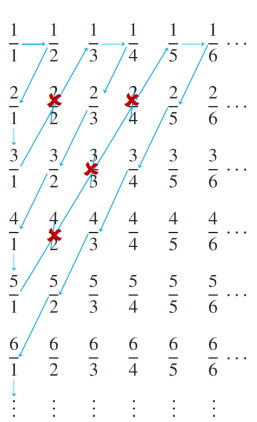
\includegraphics[width=0.3\linewidth]{qpluscountable.png} \\
    \end{center}
    This function will be a bijection from $|\mathbb{Z}^+|$ to $|\mathbb{Q}^+|$.
    \item $\mathbb{Z}^+ \times \mathbb{Z}^+$ is countable: Similar to the previous proof, but it is $(x, y)$ instead of $\frac{x}{y}$. The function $f(x, y) = \frac{(x+y-2)(x+y-1)}{2} + x$ can be used.
    \item Lemma 9.4 Proof: Use sequence argument, alternatively take an element from each set.
    \item Cardinality of $|\mathbb{R}| = |(0, 1)|$: Let $F(x)$ be the projection of $x$ from the topmost point of the circle onto the number line.
    \begin{center}
        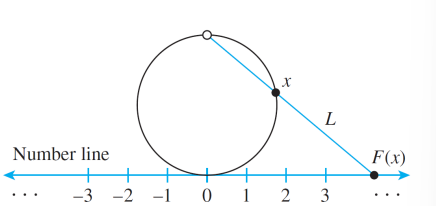
\includegraphics[width=0.5\linewidth]{realcardinality.png} \\
    \end{center}
    If points on the circle represent $(0, 1)$, then $F(x)$ is a bijection from $(0, 1)$ to $\mathbb{R}$.
\end{itemize}

\section{10./11. Counting and Probability I and II}
\subsection{Definitions}
\begin{itemize}
    \item Random Process: One outcome from a set of outcomes is guaranteed to occurr, but it is impossible to predict with certainty which outcome that will be.
    \item Sample Space: Set of all possible outcomes of a random process.
    \item Event: Subset of sample space.
    \item Equally Likely Probability: $P(E) = \frac{|E|}{|S|}$ where $E$ is an event in a finite sample space $S$.
    \item Theorem 9.1.1 Number of Elements in a List: There are $n-m+1$ integers from $m$ to $n$ inclusive, where $m \leq n$.
    \item Theorem 9.2.1 Multiplication / Product Rule: If an operation has $k$ steps and each step $i$ can be completed in $n_i$ ways, the entire operation can be completed in $n_1 \cdot n_2 \cdot ... \cdot n_k$ ways.
    \item Theorem 9.2.2 Permutations: A set of $n$ elements has $n!$ permutations.
    \item r-permutation: An r-permutation of a set with $n$ elements is an ordered selection of $r$ elements taken from the set, a.k.a $nPr$.
    \item Theorem 9.2.3 r-permutations from a set of $n$ elements: $nPr = n(n-1)(n-2)...(n-r+1) = \frac{n!}{(n-r)!}$.
    \item Theorem 9.3.1 Addition Rule: A set $A$ which is the union of $k$ mutually disjoint subsets fulfills $|A|=|A_1|+|A_2|+...+|A_k|$.
    \item Theorem 9.3.2 Difference Rule: If $B \subseteq A$, $|A \setminus B| = |A|-|B|$.
    \item Probability of Complement: $P(\bar{A})=1-P(A)$.
    \item Theorem 9.3.3 Principle of Inclusion and Exclusion: $|A \cup B| = |A|+|B|-|A \cap B|$, $|A \cup B \cup C|=|A|+|B|+|C|-|A \cap B|-|A \cap C|-|B \cap C|+|A \cap B \cap C|$. This can be extended to any finite number of sets.
    \item Pigeonhole Principle: A function from one finite set to another smaller finite set cannot be one-to-one. There must be at least 2 elements in the domain that share the same image in the co-domain.
    \item Generalised Pigeonhole Principle: For a function $f$ from a set $X$ with $n$ elements to a set $Y$ with $m$ elements, for $k < n/m$, there is some $y \in Y$ such that $y$ is the image of at least $k+1$ distinct $x \in X$.
    \item r-combination: An r-combination of a set with $n$ elements is a subset of $r$ of the $n$ elements, a.k.a $n \choose r$ or $nCr$.
    \item Formula for $n \choose r$: ${n \choose r} = \frac{nPr}{r!} = \frac{n!}{r!(n-r)!}$. In other words, $nPr = nCr \cdot r!$.
    \item Theorem 9.5.2 Permutations with Sets of Indistinguishable Objects: Suppose there are $n$ objects, with $n_i$ of $k$ different types $i$, and $n_1+n_2...+n_k =n$. The number of distinguishable permutations is $\frac{n!}{n_1!n_2!...n_k!}$.
    \item Multiset: An r-combination with repetition allowed. We can use $[]$ instead of $\{\}$ to represent a multiset.
    \item Theorem 9.6.1 Number of r-combinations with Repetition: The number of r-combinations with repetition from a set of $n$ elements is $r+n-1 \choose r$.
    \item Theorem 9.7.1 Pascal's Formula: ${n+1 \choose r} = {n \choose r-1}+{n \choose r}$.
    \item Theorem 9.7.2 Binomial Theorem: $(a+b)^n=\sum_{k=0}^{n}{n \choose k}a^{n-k}b^k$.
    \item Probability Axioms:
    \begin{itemize}
        \item $0 \leq P(A) \leq 1$
        \item $P(\emptyset)=0$ and $P(S)=1$ where $S$ is the sample space.
        \item If $A$ and $B$ are disjoint events, $P(A \cup B) = P(A)+P(B)$.
    \end{itemize}
    \item Probability of General Union of Two Events: $P(A \cup B)=P(A)+P(B)-P(A \cap B)$.
    \item Expected Value: The expected value of a process is $\sum_{k=1}^na_kp_k$ where $a_k$ is a real number and $p_k$ is the probability of $a_k$ happening.
    \item Linearity of Expectation: $E[X+Y] = E[X]+E[Y]$, regardless of whether $X$ and $Y$ are independent.
    \item Conditional Probability: The probability of $B$ given $A$ is $P(B|A)=\frac{P(A \cap B)}{P(A)}$.
    \item Theorem 9.9.1 Baye's Theorem: Suppose $S$ is the union of mutually disjoint events $B_1,B_2, ..., B_n$. If $A$ is an event in $S$, $P(B_k|A)=\frac{P(A|B_k) \cdot P(B_k)}{P(A|B_1) \cdot P(B_1) + P(A|B_2) \cdot P(B_2) + ... + P(A|B_n) \cdot P(B_n) }$
    \item Independent Events: $A$ and $B$ are independent iff $P(A \cap B) = P(A) \cdot P(B)$. Then $P(A|B)=P(A)$ and $P(B|A)=P(B)$.
    \item Pairwise Independent: Any 2 chosen events are independent.
    \item Mutually Independent: ALL events together are independent. $P(A_1 \cap A_2 \cap ... \cap A_n)=P(A_1) \cdot P(A_2) \cdot ... \cdot P(A_n)$.
\end{itemize}

\subsection{Medical Testing}
\begin{itemize}
    \item False Positive: Patient does not have disease but tests positive.
    \item False Negative: Patient has disease but tests negative.
    \item True Positive Rate / Sensitivity: $P(Test Postive | Infected)$.
    \item True Negative Rate / Specificity: $P(Test Negative | Not Infected)$.
    \item $P(Disease|+)=\frac{P(+|Disease) \cdot P(Disease)}{P(+)}$.
    \item $P(+|\overline{Disease})=\frac{P(\overline{Disease}|+) \cdot P(+)}{P(\overline{Disease})}$.
\end{itemize}

\subsection{Stars and Bars}
\begin{itemize}
    \item The number of solutions to $x_1+x_2+..+x_k=n$ where all $x_i$ are positive is $n-1 \choose k-1$. There are $n-1$ gaps between stars, $k-1$ of which need to contain bars.
    \item The number of solutions to $x_1+x_2+..+x_k=n$ where all $x_i$ are non-negative is $n+k-1 \choose k-1$. There are $n+k-1$ total stars and bars, out of which $k-1$ have to be bars.
\end{itemize}

\section{12. Graphs}
\subsection{Definitions}
\begin{itemize}
    \item Undirected Graph: An undirected graph $G$ consists of 2 finite sets: A nonempty set $V$ of vertices and a set $E$ of edges where each edge is a set consisting of either 1 or 2 vertices as endpoints. An edge connects 2 endpoints. 2 vertices connected by an edge are adjacent, and a vertex with a loop is adjacent to itself. An edge can be represented as $e=\{v, w\}$.
    \item Directed Graph: Similar to undirected graph, but each edge has an ordered pair of endpoints. A directed edge can be represented as $e=(v,w)$.
    \item Four-Colour Theorem: Four colours are sufficient to colour any map in a plane such that regions with a common boundary do not share the same colour.
    \item Simple Graph: An undirected graph with no loops are parallel edges.
    \item Complete Graph: A complete graph on $n$ vertices, $K_n$, is a simple graph with with exactly one edge connecting each pair of distinct vertices.
    \item Bipartite Graph: A simple graph whose vertices can be divided into two disjoin sets such that every edge connects 2 vertices from different sets.
    \item Complete Bipartite Graph: A bipartite graph between $U$ and $V$ such that every vertex in $U$ connects to every vertex in $V$. If $|U|=m$ and $|V|=n$, it is known as $K_{m,n}$.
    \item Subgraph: $H$ is a subgraph of $G$ iff every vertex and edge in $H$ is also in $G$.
    \item Degree: The degree of a vertex is the number of edges incident on it. An edge which is a loop is counted twice.
    \item Theorem 10.1.1 Handshake Theorem: The total degree of $G = 2 \cdot |E|$.
    \item Corollary 10.1.1: The total degree of a graph is even.
    \item Proposition 10.1.3: In any graph there are an even number of vertices of odd degree.
    \item Indegree and Outdegree of Directed Graph: The indegree of $v$, $deg^-(v)$ is the number of directed edges ending at $v$. The outdegree of $v$, $deg^+(v)$ is the number of directed edges starting at $v$. The total indegree must be the same as the total outdegree and the number of edges.
    \item Walk: An alternating sequence of adjacent vertices and edges of a graph. The number of edges is the length of the walk.
    \item Trivial Walk: A walk from a vertex to itself.
    \item Trail: A walk without a repeated edge.
    \item Path: A trail without repeated vertices.
    \item Closed Walk: Starts and ends at the same vertex.
    \item Circuit / Cycle: A closed walk of at least length 3 with no repeated edges.
    \item Simple Cycle: Cycle without any repeated vertex except first and last.
    \item Cyclic: Consists a loop or cycle, if not it is acyclic.
    \item Connectedness: 2 vertices are connected iff there is a walk between them. A graph is connected iff any 2 vertices are connected.
    \item Lemma 10.2.1: Let $G$ be a graph.
    \begin{itemize}
        \item If $G$ is connected, any two distinct vertices of $G$ can be connected by a path.
        \item If two vertices are part of a cycle in $G$ and one edge is removed from the cycle, there still exists a trail between them.
        \item If $G$ is connected and $G$ contains a cycle, an edge of the cycle can be removed without disconnecting $G$.
    \end{itemize}
    \item Connected Component: $H$ is a connected component of $G$ iff $H$ is a subgraph of $G$, $H$ is connected, and there is no connected subgraph of $G$ with $H$ as a subgraph that $\neq H$.
    \item Euler Circuit: An Euler circuit is a circuit that contains every vertex and traverses every edge exactly once.
    \item Eulerian Graph: A graph with an Euler circuit.
    \item Theorem 10.2.2: If an graph has an Euler circuit, then every vertex of the graph has a positive even degree.
    \item Contrapositive of Theorem 10.2.2: If a vertex in a graph has odd degree, the graph does not have an Euler circuit.
    \item Theorem 10.2.3: If a graph is connected and every vertex has a positive even degree, the graph has an Euler circuit.
    \item Theorem 10.2.4: A graph has an Euler circuit iff the graph is connected and every vertex has a positive even degree.
    \item Euler Trail: An Euler trail/path is a sequence of edges and vertices between 2 nodes which passes through every vertex at least once, and every edge exactly once.
    \item Corollary 10.2.5: There is an Euler trail between 2 vertices iff the graph is connected, the start and endpoints have odd degreee while all other vertices have a positive even degree.
    \item Hamiltonian Circuit: A simple circuit that includes every vertex of a graph. Every vertex appears exactly once except for the start and endpoint which are the same.
    \item Hamiltonian Graph: A graph with a Hamiltonian circuit.
    \item Proposition 10.2.6: If a graph $G$ has a Hamiltonian circuit, then $G$ has a subgraph $H$ where
    \begin{itemize}
        \item $H$ contains every vertex of $G$
        \item $H$ is connected
        \item $H$ has the same number of edges as vertices
        \item Every vertex of $H$ has degree 2.
    \end{itemize}
    \item Matrix: An $m$ by $n$ matrix has $m$ rows and $n$ columns. $a_{ij}$ is the element in the $i$th row and $j$th column.
    \item Adjacency Matrix: The $n$ by $n$ matrix where $a_{ij}$ is the number of edges from $v_i$ to $v_j$.
    \item Symmetric Matrix: $a_{ij} = a_{ji}$.
    \item Scalar Product: $\sum_{k=1}^n a_{ik}b_{kj}$.
    \item Matrix Multiplication: If $A$ is an $m$ by $k$ matrix and $B$ is an $k$ by $n$ matrix, $AB$ is the matrix where $c_{ij}=\sum_{r=1}^k a_{ir}b_{rj}$ $\forall i \leq m$ and $\forall j \leq n$.
    \item Identity Matrix: A square matrix where all entries are 0 except those on the main diagonal which are 1.
    \item nth Power of a Matrix: $A^0=I$ where $I$ is the identity matrix, $A^n=AA^{n-1}$.
    \item Theorem 10.3.2: The $ij$th entry of $A^n =$ number of walks of length $n$ from $v_i$ to $v_j$.
    \item Isomorphic Graph: 2 graphs are isomorphic iff there exists bijections between their vertices and edges which preserve the edge-endpoint functions. For simple graphs, 2 graphs are isomorphic iff there exists a permutation of vertices which preserves edges.
    \item Theorem 10.4.1 Graph Isomorphism is an Equivalence Relation.
    \item Planar Graph: A graph that can be drawn on a two dimensional plane without edges crossing.
    \item Kuratowski's Theorem: A finite graph is planar iff it does not contain a subgraph that is a subdivision of the complete graph $K_5$ or the complete bipartite graph $K_{3,3}$.
    \item Euler's Formula: A connected planar graph has $f=e-v+2$ faces.
\end{itemize}

\subsection{Graph Notes}
\begin{itemize}
    \item An Euler circuit may visit some vertices more than once so it might not be a Hamiltonian circuit.
    \item A Hamiltonian circuit might not include all edges and hence may not be an Euler circuit.
    \item For an undirected graph, the adjacency matrix is symmetric.
    \item For matrix multiplication, $c_{ij}$ is the scalar product of the $i$th row of $A$ and the $j$th column of $B$.
    \item Matrix multiplication is NOT commutative!
\end{itemize}

\section{13. Trees}
\subsection{Definitions}
\begin{itemize}
    \item Tree: A tree is a simple graph iff it is simple, acyclic, and connected.
    \item Trivial Tree: Tree with one vertex.
    \item Forest: A graph is a forest iff it is simple, acyclic, and not connected.
    \item Lemma 10.5.1: Any non-trivial tree has at least one vertex f degree 1.
    \item Terminal Vertex (Leaf) and Internal Vertex: A vertex in a tree with degree 1 is a leaf, a vertex with degree more than 1 is an internal vertex.
    \item Theorem 10.5.2: Any tree with $n$ vertices has $n-1$ edges.
    \item Lemma 10.5.3: If a graph is connected, removing an edge from a cycle in the graph keeps the graph still connnected.
    \item Theorem 10.5.4: If a connected graph has $n$ vertices and $n-1$ edges, the graph is a tree.
    \item Rooted Tree: A rooted tree has a specific vertex designated as the root.
    \item Level: The level of a vertex is the number of edges along the unique path between it and the root.
    \item Height: The height of a rooted tree is the maximum level of any vertex of the tree.
    \item Child: The children of a vertex are adjacent to it and are one level farther from the root.
    \item Parent: If $w$ is a child of $v$, $v$ is the parent of $w$.
    \item Siblings: Two vertices with the same parent are known as siblings.
    \item Ancestor and Descendant: If $v$ lies on the unique path between $w$ and the root, $v$ is an ancestor of $w$, and $w$ is a descendant of $v$.
    \item Binary Tree: A binary tree is a rooted tree where every parent has at most two children. Each child is either a left or right child.
    \item Full Binary Tree: A binary tree where each parent has exactly two children.
    \item Left / Right Subtree: The left subtree of a vertex is the binary tree whose root is the left child of the vertex, with vertices which are descendants of the left child and edges connecting vertices in the left subtree. The right subtree is defined analogously.
    \item Theorem 10.6.1 Full Binary Tree: A full binary tree with $k$ internal vertices has $2k+1$ total vertices and $k+1$ terminal vertices.
    \item Theorem 10.6.2 Height of Binary Tree: For a binary tree with height $h$ and $t$ leaves, $t \leq 2^h$ and $log_2t\leq h$.
    \item Breadth-First-Search: Start at the root, visit adjacent vertices, then move to the next level.
    \item Depth-First Search:
    \begin{itemize}
        \item Pre-Order: Print Self, Traverse Left, Traverse Right
        \item In-Order: Traverse Left, Print Self, Traverse Right
        \item Post-Order: Traverse Left, Traverse Right, Print Self
        \item Follow the path around the nodes, and write down a node when the circle on it is met.
        \item Given only pre-order and post-order, there might be more than one tree that satisifes.
    \end{itemize}
    \item Spanning Tree: A subgraph that contains every vertex, and is a tree.
    \item Proposition 10.7.1: Every connected graph has a spanning tree, and any two spanning trees for a graph have the same number of edges.
    \item Weighted Graph: A graph where every edge has a positive real number weight.
    \item Minimum Spanning Tree: A spanning tree with the least possible total weight.
    \item Kruskal's Algorithm:
    \begin{itemize}
        \item Process edges in order of increasing weight.
        \item If an edge does not produce a cycle, add it to the minimum spanning tree.
    \end{itemize}
    \item Prim's Algorithm:
    \begin{itemize}
        \item Create a graph with a starting vertex, and consider the set of vertices of the graph excluding the start point.
        \item Find an edge connecting the current graph to one of the remaining vertexes with least weight.
        \item Add this edge and its endpoints to the current graph.
    \end{itemize}
    \begin{center}
        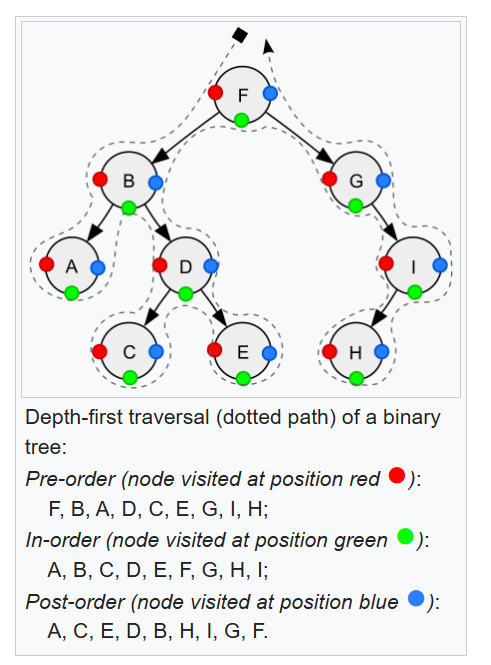
\includegraphics[width=0.5\linewidth]{dfs.png}
    \end{center}
\end{itemize}

\section{Useful Tutorial Questions}
\begin{itemize}
    \item Tutorial 1 Question 10: The product of any two odd integers is an odd integer.
    \item Tutorial 1 Question 11: $n^2$ is odd iff $n$ is odd. $n^2$ is even iff $n$ is even.
    \item Tutorial 2 Question 4: Rational numbers are closed under addition. Integers and rational numbers are not closed under division.
    \item Tutorial 2 Question 11: If $n = ab$ where $a$ and $b$ are positive, then $a \leq n^\frac{1}{2}$ or $b \leq n^\frac{1}{2}$.
    \item Tutorial 3 Question 5: $A \cap (B \backslash C) = (A \cap B) \backslash C$.
    \item Tutorial 3 Question 6: $A \backslash (B \backslash C) = (A \backslash B) \cup (A \cap C)$.
    \item Tutorial 3 Question 8: $A \subseteq B$ iff $A \cup B = B$.
    \item Tutorial 3 Question 9: $(A \backslash B) \cup (B \backslash A) = (A \cup B) \backslash (A \cap B)$.
    \item Tutorial 4 Question 2: Show the following are logically equivalent: (i) R is symmetric, (ii) $\forall x, y \in A, x R y \leftrightarrow y R x$, (iii) $R = R^{-1}$.
    \begin{itemize}
        \item (i) $\rightarrow$ (ii)
        \begin{itemize}
            \item Suppose $R$ is symmetric
            \item Let $x, y \in A$
            \item If $x R y$ then $y R x$ by symmetry of $R$
            \item If $y R x$ then $x R y$ by symmetry of $R$
            \item $\therefore x R y \leftrightarrow y R x$
        \end{itemize}
        \item (ii) $\rightarrow$ (iii)
        \begin{itemize}
            \item Suppose $\forall x, y \in A, x R y \leftrightarrow y R x$
            \item $\forall x, y \in A$
            \item $(x, y) \in R \leftrightarrow x R y$ by definition of $x R y$
            \item $\leftrightarrow y R x$
            \item $\leftrightarrow x R^{-1} y$ by definition of $R^{-1}$
            \item $\leftrightarrow (x, y) \in R^{-1}$ by definition of $x R^{-1} y$
            \item $\therefore R = R^{-1}$
        \end{itemize}
        \item (iii) $\rightarrow$ (i)
        \begin{itemize}
            \item Suppose $R = R^{-1}$
            \item Let $x, y \in A, x R y$
            \item Then $x R^{-1} y$ as $R = R^{-1}$
            \item $y R x$ by definition of $R^{-1}$
            \item $\therefore$ R is symmetric
        \end{itemize}
    \end{itemize}
    \item Tutorial 4 Question 5: For an equivalence relation $R$,
    \begin{itemize}
        \item (i) $R^{-1} \circ R = R \circ R^{-1}$
        \item (ii) $R \subseteq R \circ R$
        \item (iii) $R \circ R \subseteq R$
        \item (iv) $R \circ R^{-1} = R$
        \item (v) $R = R \circ R$ from (ii) and (iii)
    \end{itemize}
    \item Tutorial 4 Question 7: Composition of relations is associative, $T \circ (S \circ R) = (T \circ S) \circ R$.
    \item Tutorial 5 Question 5: $\subseteq$ on $\mathcal{P}(A)$ is a partial order.
    \item Tutorial 5 Question 8: Every asymmetric relation is antisymmetric.
    \item Tutorial 5 Question 11: Any two comparable elements are compatible. Any two compatible elements are not necessarily compatible.
    \item Tutorial 6 Question 4: $(g \circ f)^{-1} = f^{-1} \circ g^{-1}$.
    \item Tutorial 6 Question 6:
    \begin{itemize}
        \item Given $f : A \rightarrow B$
        \item $g : B \rightarrow A$ is a left inverse of $f$ iff  $g(f(a)) = a$ $\forall a \in A$
        \item $h : B \rightarrow A$ is a left inverse of $f$ iff  $f(h(b)) = b$ $\forall b \in B$
        \item The statement if a function has a left inverse, then it has a right inverse, is false. The converse is also false.
    \end{itemize}
    \item Tutorial 6 Question 7: Let $f : B \rightarrow C$. Given a function $g$ with domain $C$ such that $g \circ f$ is injective, $f$ is injective.
    \item Tutorial 6 Question 9: Considering preimage and image:
    \begin{itemize}
        \item $X \subseteq f^{-1}(f(X))$, but not necessarily $f^{-1}(f(X)) \subseteq X$.
        \item $Y \subseteq f(f^{-1}(Y))$, but not necessarily $f(f^{-1}(Y)) \subseteq Y$.
    \end{itemize}
    \item Tutorial 6 Question 10: For the relation $x \sim y \leftrightarrow x-y \in \mathbb{Z}$ on $\mathbb{Q}$, red addition is well-defined while red-multiplication is not well-defined.
    \item Tutorial 7 Question 2: $\sum_{k=1}^n k^2=\frac{1}{6}n(n+1)(2n+1)$.
    \item Tutorial 7 Question 3: $1+nx \leq (1+x)^n$ for $n \in \mathbb{Z}^+$ and $x \in \mathbb{R}_{\geq -1}$.
    \item Tutorial 7 Question 4: Given odd $a$, $2^{n+2} | (a^{2^n}-1)$.
    \item Tutorial 7 Question 5: Any number $\geq 8$ can be made up of multiple 3's and 5's.
    \item Tutorial 7 Question 6: Every positive integer can be written as a sum of distinct non-negative integer powers of 2.
    \item Tutorial 7 Question 7: Given $a_0=0, a_1=2, a_2=7, a_{n+3}=a_{n+2}+a_{n+1}+a_n$, $a_n < 3^n$.
    \item Tutorial 7 Question 8: For the Fibonacci function, $F(a+b)=F(a+1) \cdot F(b) + F(a) \cdot F(b-1)$. To prove this, use the base cases $P(0, b)$ and $P(1, b)$.
    \item Tutorial 7 Question 9: Hamming numbers defined by $1 \in H$ and $n \in H \rightarrow 2n \in H, 3n \in H, 5n \in H$, have a canonical representation; a unique way of representing each member of the set as $2^i3^j5^k$.
    \item Tutorial 8 Question 1: $\mathbb{Z}$ is countable using the formula $g(n)=(-1)^n \lfloor x \rfloor$.
    \item Tutorial 8 Question 2: The union of a countably infinite set and a finite set is countable. Create a new sequence with all elements of the finite set in front.
    \item Tutorial 8 Question 3: The union of infinitely many finite sets is infinite.
    \item Tutorial 8 Question 4: The union of a finite number of countable sets is countable.
    \item Tutorial 8 Question 5: Let $S_i$ be a countably infinite set for each $i \in \mathbb{Z}^+$. The union of all $S$ is countable. This can be proven by using the fact that $\mathbb{Z}^+ \times \mathbb{Z}^+$ is countable.
    \item Tutorial 8 Question 6: A bijection exists between $X \cup Y$ and $X$ where $X$ is an infinite set and $Y$ is a finite set.
    \item Tutorial 8 Question 7: The power set of a countably infinite set is uncountable. This can be proven by a diagonalisation argument.
    \begin{itemize}
        \item Suppose $\mathcal{P}(A)$ is countable.
        \item $\mathcal{P}(A)$ is infinite as $A$ is infinite.
        \item There is a sequence $a$ where every element of $A$ appears exactly once.
        \item There is a sequence $B$ where every element of $\mathcal{P}(A)$ appears exactly once.
        \item Now define $B=\{a_i:a_i \notin b_i\}$.
        \item Note that $B\in\mathcal{P}(A)$.
        \item Then $B\neq B_i$ for all $i$.
        \item This is because if $a_i\notin B_i$, then $a_i\in B$, and if $a_i\in B_i$, then $a_i \notin B$. So in all cases, $B\neq B_i$.
        \item Since $B$ is not in the original sequence, this contradicts the claim that $\mathcal{P}(A)$ is countable.
        \item Therefore $\mathcal{P}(A)$ is uncountable.
    \end{itemize}
    \item Tutorial 8 Question 8: If R is reflexive, then $|A| \leq |R|$. The same i snot necessarily true for symmetry and transitivity.
    \item Tutorial 8 Question 9: $Even(F_n) \leftrightarrow Even(F_{n+3})$.
    \item Tutorial 8 Question 10: Given the equivalence relation $g(a) = g(b) \leftrightarrow a \sim b$, the function $f : X/\sim \rightarrow Y$ given by $f([x]) = g(x)$ is well-defined and injective.
    \item Tutorial 9 Question 4: Given $n$ boxes with white or blue balls, such that at least one box contains a white ball, and boxes with white balls are consecutive, this can be done in $\frac{n(n+1)}{2}$ ways. For $1 \leq k \leq n$, there are $n-k+1$ ways.
    \item Tutorial 9 Question 5: The number of circular permutations of $n$ objects is $(n-1)!$.
    \item Tutorial 9 Question 9:
    \begin{itemize}
        \item If you randomly put 51 points in a unit square, there are always 3 points that can be covered by a circle with radius 1/7.
        \item Divide the unit square into 25 equal smaller squares. One small square must have at least three points. 
        \item The diagonal of the square is less than the diameter of the circle we want to place, so it can be fully contained.
    \end{itemize}
    \item Tutorial 9 Question 10: Given any 5 distinct non-negative integers, two of them have a difference divisible by 4.
    \item Tutorial 9 Question 11:
    \begin{itemize}
        \item A chessmaster has 11 weeks to prepare for a tournament. They play at least 1 game every day, but no more than 12 games in any week. There is a succession of consecutive days where the chess master will have played exactly 21 games.
        \item Consider 77 days, and $P_i$ as the cumulative number of games played including day $i$. All $1 \leq P_i \leq 132$, and are distinct. 
        \item Consider $Q_i = P_i+21$. The largest $Q_i$ possible is 153, and they are also distinct. 
        \item There are 154 possible numbers, but the range of $P_i$ and $Q_i$ is 153. There must be some $P_j=Q_i=P_i+21$.
        \item The chess master plays exactly 21 games from day $i+1$ to $j$.
    \end{itemize} 
    \item Tutorial 10 Question 2: From Tutorial 9 Question 4: Put crosses on the side of all boxes. Choose 2 out of $n+1$ crosses to be the start and end of boxes with white balls. The number of ways is ${n+1 \choose 2} = \frac{n(n+1)}{2}$.
    \item Tutorial 10 Question 6: For a random relation on a power set, what is the probability that the relation is:
    \begin{itemize}
        \item Reflexive: Consider the $n$ by $n$ matrix. For a reflexive relation, all entries in the diagonal must be 1. For the remaining $n^2-n$ entries, they can be anything we wish. So $P(Reflexive)=\frac{2^{n^2-n}}{2^{n^2}}=\frac{1}{2^n}$.
        \item Symmetric: Consider the $n$ by $n$ matrix. For a symmetric relation, $a_{ij} = a_{ji}$. We can consider the lower triangular half of the matrix and the main diagonal, and let these be anything we want. There are $\frac{n^2+n}{2}$ entries, so $P(Symmetric)=\frac{2^{\frac{n^2+n}{2}}}{2^{n^2}}=\frac{1}{2^{\frac{n^2-n}{2}}}$.
        \item Antisymmetric: Entries on the main diagonal can be either 0 or 1. For a $a_{ij}$ in the lower triangular half of the matrix, there can be 3 possibilities: $i$ and $j$ are unrelated, $iRj$, or $jRi$. This gives $2^n\cdot3^{\frac{n(n-1)}{2}}$ relations, and a probability of $2^{n-n^2}\cdot3^{\frac{n(n-1)}{2}}$. 
    \end{itemize}
    \item Tutorial 10 Question 8: There are 4 non-isomorphic undirected graphs with two vertices and two edges.
    \item Tutorial 10 Question 10: Given  group of people who shake hands including a host who shook hand with everyone else, there are at least two people who shook hands the same number of times.
    \item Tutorial 10 Question 11: A dominating set is a set of vertices in an undirected simple graph where every vertex outside of this set is adjacent to at least one vertex in this set. A minimal dominating set does not have a dominating proper subset.
    \item Tutorial 10 Question 11: For all simple graphs with 6 vertices, either the graph or its complement contains a triangle.
    \item Tutorial 11 Question 4: If a simple undirected graph is connected, then $|E| \geq |V|-1$. The converse is NOT true.
    \item Tutorial 11 Question 5: If a simple undirected graph is acyclic, then $|E| \leq |V|-1$. The converse is NOT true.
    \item Tutorial 11 Question 6: For a simple undirected graph, it is a tree iff there is exactly one path betewen every pair of vertices.
    \item Tutorial 11 Question 7: If separating stones into 2 piles gives $k_1\times k_2$ money, the maximum (only) amount of money you can earn is $\frac{n(n-1)}{2}$. Imagine splitting as cutting all edges in the bipartite graph between the 2 resulting sets. Since every edge has to be cut, the total is the number of edges in the complete graph.
    \item Tutorial 11 Question 9: Number of binary trees with $n$ nodes is the $n$th Catalan Number. $C_n=\frac{1}{n+1}{2n \choose n}$. $C_i=1, 2, 5, 14, 42, 132$.
\end{itemize}

\section{Useful Assignment Questions}
\begin{itemize}
    \item Assignment 1 Question 1: Variant Absorption Laws
    \begin{itemize}
        \item $p \land (\lnot p \lor q)\equiv p\land q$
        \item $p \lor (\lnot p \land q)\equiv p \lor q$
    \end{itemize}
    \item Assignment 1 Question 6(b): $A \subseteq \emptyset \rightarrow A = \emptyset$.
    \item Assignment 1 Question 6(c): $\mathcal{P}(A\cap B)=\mathcal{P}(A)\cap\mathcal{P}(B)$.
    \item Assignment 2 Question 2(c): On average how many times must a 6-sided fair dice be rolled until a 3 turns up? $E(X)=\frac{1}{6}\cdot 1+\frac{5}{6}(E(X)+1)$, giving $E(X)=6$.
    \item Assignment 2 Question 5: $14 | 2^{4n}-2^n$.
    \item Assignment 2 Question 6: Let $f:\mathcal{P(\mathbb{N})\backslash\{\emptyset\}}\to\mathbb{N}$ map $S$ to its smallest element. Then, $f$ does not have an inverse, and $f^{-1}(\{n\})$ is uncountable.
\end{itemize}

\end{multicols*}

\clearpage
\begin{figure}
    \clearpage
    \centering
    
\includegraphics[width=\textwidth]{tantc.jpg}
    pls give me A+ prof thanks
\end{figure}

\end{document}